\documentclass{article}
\usepackage[a4paper, margin=1in]{geometry}
\usepackage[utf8]{inputenc}
\usepackage[russian]{babel}

\usepackage[nottoc,numbib]{tocbibind}
\usepackage{graphicx}
\usepackage{wrapfig}
\usepackage{subcaption}
\usepackage{amsmath}

\graphicspath{{./images/}}

\title{Математические методы в робототехнике}
\author{
Чистый Аркадий\\
Хохлов Николай\\
Молчанов Егор\\
Научный руководитель: Мисюрин Сергей Юрьевич
}
\date{2020 - 2021}



\begin{document}
\begin{center}
МИНИСТЕРСТВО НАУКИ И ВЫСШЕГО ОБРАЗОВАНИЯ РОССИЙСКОЙ ФЕДЕРАЦИИ
\vfill
Федеральное государственное автономное образовательное учреждение высшего образования\\
\bigskip
Национальный исследовательский ядерный университет «МИФИ»
\vfill
ИНСТИТУТ ИНТЕЛЛЕКТУАЛЬНЫХ КИБЕРНЕТИЧЕСКИХ СИСТЕМ
\vfill
Направление подготовки: 01.03.02 Прикладная математика и информатика
\vfill
ПРОЕКТНАЯ ПРАКТИКА
\vfill
{\large Пояснительная записка к проекту

\medskip
{\bfseries \Large «Математические методы в робототехнике»}}
\vfill
\end{center}
\begin{flushright}
Выполнили:\\
	Чистый Аркадий, Б19-511\\
	Хохлов Николай, Б19-501\\
	Молчанов Егор, Б19-501\\
\medskip
Научный руководитель:\\
	Мисюрин Сергей Юрьевич
\end{flushright}
\vfill
\vfill
\begin{center}
Москва, 22 декабря 2020 года
\end{center}
\vfill
\vfill
\pagebreak

\tableofcontents
\newpage

\section{Введение}
Существует множество алгоритмов передвижения робота. Большинство из них подходит для широкого спектра роботов. Однако для тяжёлых роботов многие алгоритмы плохо оптимизированы. Таким образом, для подобных роботов приходиться подбирать оптимальный алгоритм и его параметры так, чтобы добиться нужных результатов.

\section{Постановка задачи}
Основная цель - достичь высокой скорости реальным шестиногим роботом. Робот имеет относительно большую массу (2.3 кг), поэтому стоит вопрос выбора алгоритма его передвижения.

В работах \cite{ref1,ref7} указывается, что схемы передвижения Ripple Gait и Tripod Gait имеют самую высокую скорость. Необходимо их сравнить и выбрать необходимую нам схему. Затем выбранную схему необходимо оптимизировать так, чтобы скорость робота была максимальной.

\section{Схемы передвижения робота}
Схема передвижения робота - описание движения каждой его конечности при его перемещении. Известно множество схем передвижения. Задача - сравнить две самые используемые из них для шестиногого робота: Ripple Gait и Tripod Gait. Их схемы представлены на рис. \ref{fig:gaits}.

\begin{figure}[h]
	\begin{subfigure}[b]{0.5\linewidth}
		\centering
		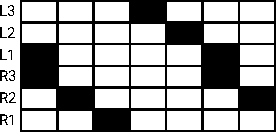
\includegraphics[height=7em]{ripple_gait}
		\caption{Ripple Gait}
		\label{fig:ripple_gait}
	\end{subfigure}
	\hfill
	\begin{subfigure}[b]{0.5\linewidth}
		\centering
		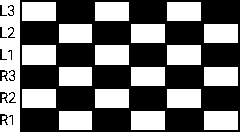
\includegraphics[height=7em]{tripod_gait}
		\caption{Tripod Gait}
		\label{fig:tripod_gait}
	\end{subfigure}
	\caption{Схемы передвижения}
	\label{fig:gaits}
\end{figure}

Схема задаётся в виде таблицы (см. рис. \ref{fig:gaits}), где чёрные ячейки - временные отрезки, в которых конечность, соответствующая данной строке находится на поверхности, а белые - в которых конечность находится над поверхностью.

\subsection{Измерение скорости робота}
Все приведённые скорости получены усреднением измерений, проведённых двумя способами.

\paragraph*{1-й способ}
Измерялось расстояние пройденное роботом и время прохождения этого расстояния. Результат получался путём деления расстояния на затраченное время.

\paragraph*{2-й способ}
Использовался встроенный в робота ультразвуковой измеритель расстояния. Проводилось две серии измерений, каждая серия состояла из 5-ти измерений по 0.01 сек., интервал между сериями - 0.5 сек. \\
Таким образом, итоговая скорость считалась по формуле $$v = \frac{S_1-S_2}{0.5\text{ сек.}}$$
где $$S_1 = \frac{\sum_{i=1}^{5} S_1^{(i)}}{5}, S_2 = \frac{\sum_{i=1}^{5} S_2^{(i)}}{5}$$
$S_1^{(i)}, S_2^{(i)}, i=1,2,\ldots,5$ - результаты измерений первой и второй серии

\subsection{Сравнение схем передвижения}

Для сравнения схем была написана программа, которая принимает на вход схему, записанную в виде текста, в котором 0 соответствуют белой клетке, 1 - чёрной. Реальный робот двигается согласно введённой схеме.

\begin{figure}[h]
	\centering
	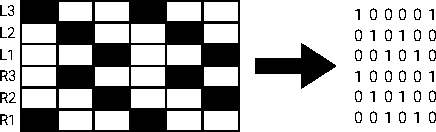
\includegraphics[height=7em]{gait_program}
	\caption{Входной формат схемы}
	\label{fig:gait_program}
\end{figure}

Сравнивались максимальные скорости, которых удавалось достичь при использовании каждой схемы без внесения существенных изменений в алгоритм передвижения.

Скорость при использовании Tripod Gait равна 22 см/с, при использовании Ripple Gait - 15 см/с. Для дальнейших совершенствований алгоритма передвижения была выбрана схема Tripod Gait.
\subsection{Оптимизация схемы Tripod Gait}

Каждая конечность задействует три сервопривода при движении. Чтобы уменьшить время, за которое конечность переходит из нижнего положения в верхнее и наоборот, а также объём вычислений необходимый для движения ноги была проведена оптимизация.

\begin{figure}[h]
	\begin{subfigure}[b]{0.48\linewidth}
		\centering
		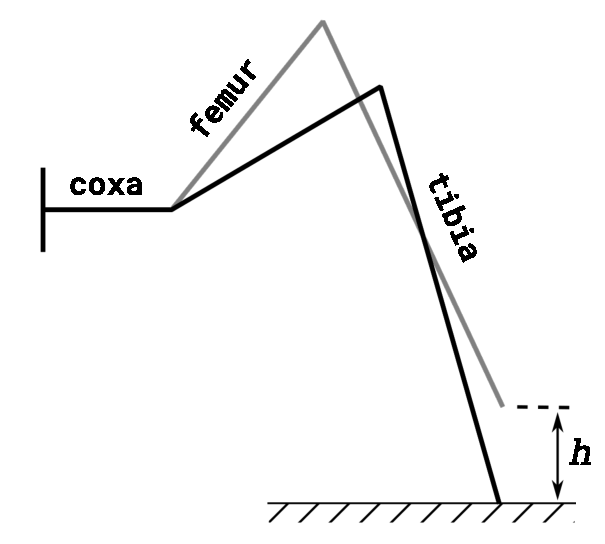
\includegraphics[height=10em]{optimize_1}
		\caption{До оптимизации}
		\label{fig:optimize_1}
	\end{subfigure}
	\hfill
	\begin{subfigure}[b]{0.52\linewidth}
		\centering
		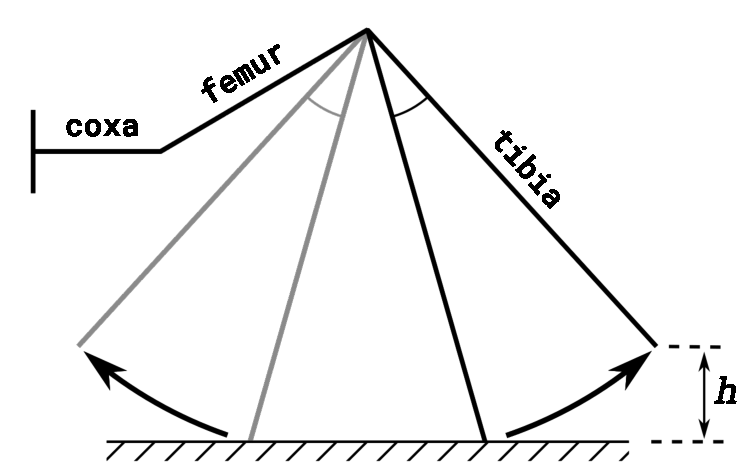
\includegraphics[height=10em]{optimize_2}
		\caption{После оптимизации}
		\label{fig:optimize_2}
	\end{subfigure}
	\label{fig:optimize}
	\caption{}
\end{figure}

\begin{wrapfigure}{l}{0.4\linewidth}
	\centering
	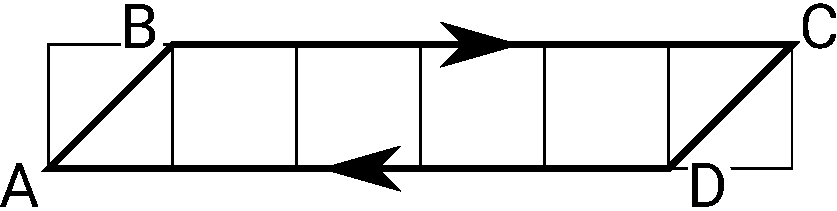
\includegraphics[height=4em]{trajectory}
	\caption{Оптимизация траектории\\(вид сбоку)}
	\label{fig:optimize_3}
\end{wrapfigure}

До оптимизации бралась точка на расстоянии $h$ выше текущей (см. рис. \ref{fig:optimize_1}), положения всех сервоприводов пересчитывались. После оптимизации для поднятия ноги работает только звено tibia (см. рис. \ref{fig:optimize_2}), потому что это звено самое лёгкое и поднимается быстрее всего. Это уменьшает объём вычислений и увеличивает максимальную скорость робота.

Также была проведена оптимизация траектории конечности - рис. \ref{fig:optimize_3}. Вместо примитивной прямоугольной траектории была взята траектория в форме параллелограмма $ABCD$. В точке $B$ конечность уже имеет некоторую начальную скорость, которая позволяет пройти отрезок над поверхностью за минимальное время. Аналогично для точки $D$: время потраченное на прохождение отрезка $DA$ будет минимальным.

\section{Математические уравнения движения механической системы}
\subsection{Уравнение Лагранжа второго рода}
Если голономная механическая система (система, механические связи которой можно свести к геометрическим) описывается лагранжианом $L(q_{i},{\dot {q}_{i}},t)$, где $q_{i}$ — обобщённые координаты, $t$ — время, точкой обозначено дифференцирование по времени) и в системе действуют только потенциальные силы, то уравнения Лагранжа второго рода имеют вид  ${\displaystyle {\frac {d}{dt}}\left({\frac {\partial L}{\partial {\dot {q}}_{i}}}\right)-{\frac {\partial L}{\partial q_{i}}}=0}$,
где $i = 1,2,\ldots,n$ ($n$ — число степеней свободы механической системы). Лагранжиан представляет собой разность кинетической и потенциальной энергий системы.

При наличии и потенциальных, и непотенциальных обобщённых сил появляется правая часть: $\displaystyle{\frac{d}{dt} (\frac{\partial L}{\partial\dot q_i})-\frac{\partial L}{\partial q_i} = R_i,\ q_{1,2,3}=\alpha,\beta,\gamma}$

\subsection{Математическое описание конкретного механизма}
\begin{wrapfigure}{l}{0.5\linewidth}
    \centering
    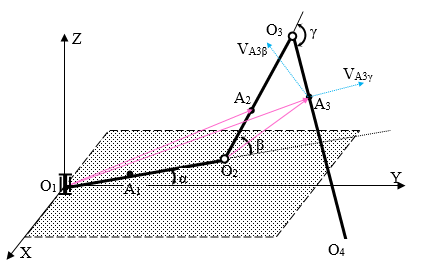
\includegraphics[width=1\linewidth]{3d}
\end{wrapfigure}

$|O_1O_2|=l_1$\\
$|O_2O_3|=l_2$\\
$|O_3O_4|=l_3$\\
$|O_1A_1|=p_1$\\
$|O_2A_2|=p_2$\\
$|O_3A_3|=p_3$\\
$|O_1A_2|=L_1$\\
$|O_1A_3|=L_2$\\
$|O_2A_3|=L_3$\\
$A_i$ --- центр тяжести звеньев\\
$m_i$ --- массы звеньев\\
$m_{g3}$ --- масса третьего ротора\\
$p_i$ --- координаты центров масс\\
$J_{Ai}$ --- момент инерции звеньев относительно центров масс\\
$J_{gi}$ --- момент инерции роторов двигателей, установленных в шарнирах звеньев\\
$M_{di}$ --- момент развиваемый двигателем\\
$M_{ci}$ --- момент сопротивления\\
$\alpha,\beta,\gamma$ --- обобщенные координаты, углы поворота звеньев, отсчитываемые согласно рисунку\\
$L = T^{(1)} + T^{(2)} + T^{(3)} - U^{(2)} - U^{(3)}$\\
$\begin{aligned}T^{(1)} &= {\frac{m_1 {V_{A1}}^2}{2}} +\frac{J_{A1}{\dot\alpha}^2}{2} + \frac{J_{g1} {\dot\alpha}^2}{2} \\&= {p_1 \dot\alpha}^2 \frac{m_1}{2} +\frac{J_{A1}}{2}{\dot\alpha}^2 +\frac{J_{g1}}{2} {\dot\alpha}^2 \\&= \frac{1}{2} ({p_1}^2 m_1 + J_{A1}+ J_{g1}){\dot\alpha}^2\end{aligned}$\\
$T^{(2)} = \frac{m_2 {V_{A2}}^2}{2} + \frac{J_{A2}}{2}({(\dot\alpha \cos\beta)}^2+{\dot\beta}^2) + \frac{J_{g2}}{2}{\dot\beta}^2$\\
$T^{(3)} = \frac{{L_2}^2 {\dot\alpha}^2 + {L_3}^2 {\dot\beta}^2 + {p_3}^2 {\dot\gamma}^2+ ({L_3}^2+{p_3}^2-{l_2}^2)\dot\beta\dot\gamma}{2}m_3 + \frac{J_{A3}}{2}({(\dot\alpha \cos{\gamma - \beta})}^2 + {(\dot\gamma -\dot\beta)}^2) +\frac{J_{g3}}{2}{\dot\gamma}^2$\\
$U_2 = m_2gp_2\sin\beta + m_{g3}l_2\sin\beta$\\
$U_3=m_3g(l_2\sin\beta - p_3\sin{(\gamma-\beta)})$\\
${L_1}^2={l_1}^2+{p_3}^2+2l_1p_2\cos(\beta)$\\
${L_2}^2={l_1}^2+{l_2}^2+{p_3}^2+2l_1l_2\cos(\beta)+2l_2p_3\cos(\gamma)+2l_1p_3\cos(\gamma-\beta)$\\
${L_3}^2={l_2}^2+{p_3}^2+2l_2p_3\cos(\gamma)$

\subsection{Численные методы решения дифференциальных уравнений}
\paragraph*{Метод Рунге-Кутты второго порядка}
Методы Рунге-Кутты --- класс численных методов решения задачи Коши для обыкновенных дифференциальных уравнений и их систем.

\noindent$y'=f(x,y),\ y(x_0)=y_0\\
y_{n+1}=y_n + \frac{h}{2}(k_1 + 2k_2 + 2k_3+k_4)\\
k_1 = f(x_n,y_n),\\
k_2=f(x_n + \frac{h}{2},y_n+\frac{h}{2}k_1),\\
k_3=f(x_n + \frac{h}{2}, y_n + \frac{h}{2}k_2),\\
k_4=f(x_n+h,y_n+hk_3).\\ \\
h\text{ --- шаг алгоритма по оси x}$


\section{Изучение программ для моделирования роботов}
\subsection{Robot Operating System (ROS)}
Robot Operating System (ROS) - это гибкий фреймворк для разработки программного обеспечения роботов. Это набор разнообразных инструментов, библиотек для упрощения задач разработки ПО роботов. Мы выбрали данную платформу для разработки модели робота ввиду его следующих возможностей и преимуществ. 
\subsubsection{Преимущества и возможности}
\begin{enumerate} 
	\item Активное и открытое сообщество\\
	Объем информации, необходимой для использования ROS достаточно велик, однако нам как незнакомым с этой областью разработчикам, получилось разобраться в этой системе, во многом потому что многие ответы на вопросы и инструкции описаны на собственном вики, которое содержит более 18000 страниц. Активные пользователи создают различные открытые пакеты, что расширяет возможности использования этой системы. 

	\item Поддержка различных языков программирования \\
	Программные модули ROS могут быть записаны на любом языке, для которого была написана клиентская библиотека. В настоящее время клиентские библиотеки существуют для C++ (roscpp), Python (rospy), Java (rosjava) и других современных языков программирования.

	\item Различные инструменты для работы\\
	ROS предлагает инструменты для 3D-визуализации (RViz) и 3D симуляции (Gazebo) - именно они использовались нами при моделировании робота-паука. 

\end{enumerate}

\subsection{Gazebo}
Gazebo - бесплатный Open Source симулятор, который предлагает возможность эффективно моделировать  роботов в сложной внутренней и внешней среде. Он отлично интегрируется с операционной системой ROS, а значит разработанную  программу управления виртуальным роботом в Gazebo и ROS будет относительно несложно перенести на реального робота.

\subsection{Модель робота паука}
\begin{wrapfigure}{L}{0.4\linewidth}
	\centering
	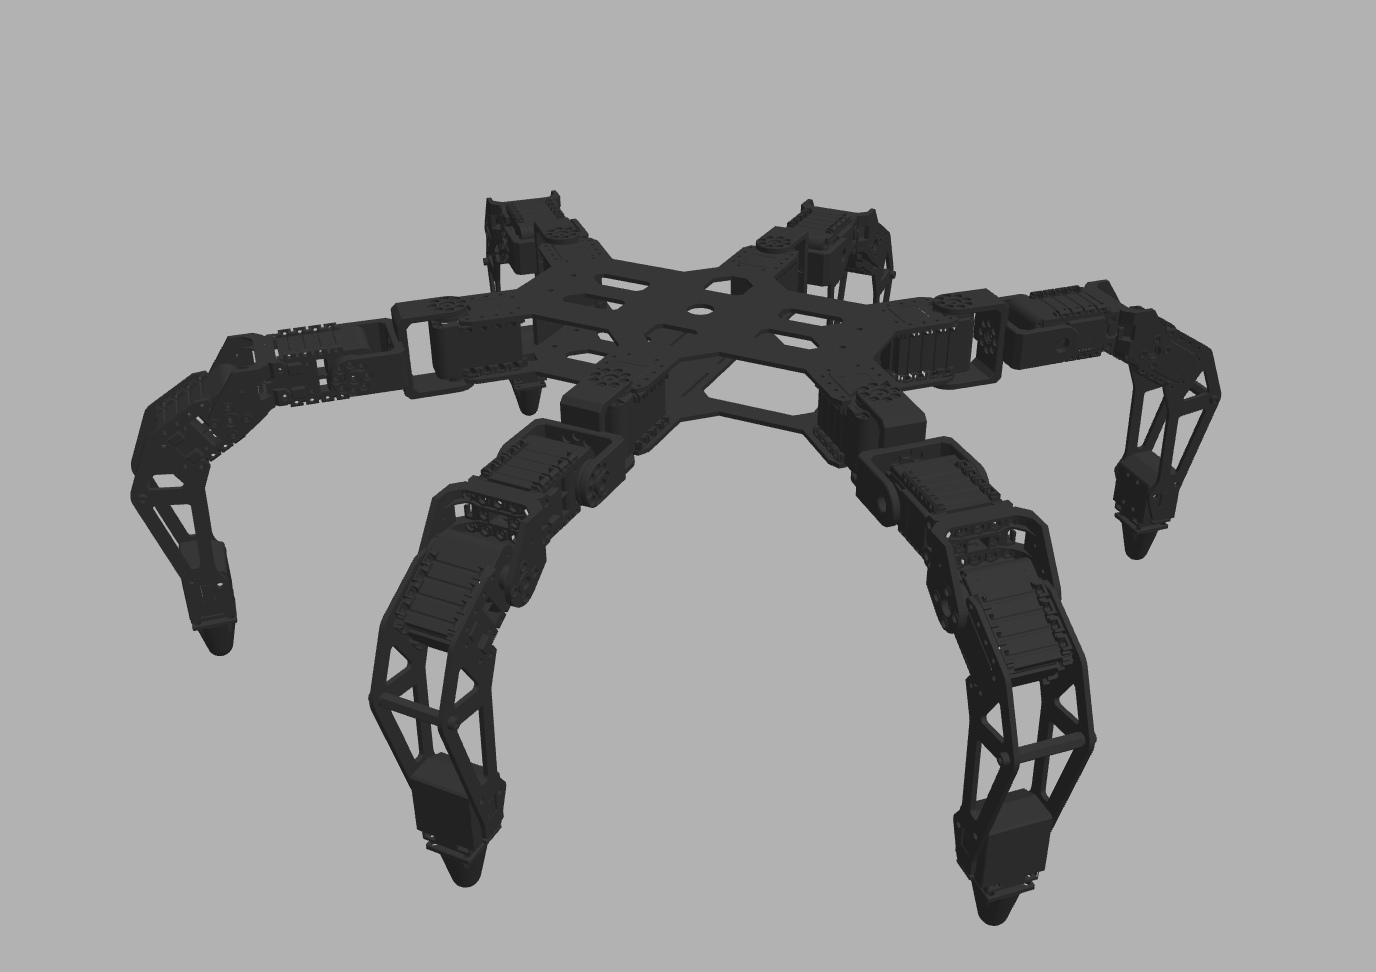
\includegraphics[height=12em]{spider_model}
	\caption{Модель робота-паука}
\end{wrapfigure}

Базовым инструментами для создания какой-либо модели в Gazebo является EditorMode, в котором доступны простые геометрические тела, такие как параллелепипед, цилиндр и шар; их можно соединять, а также устанавливать различные свойства (плотность вещества, инерция, цвет и т.д). Создание полноценной модели паука из этого набора деталей не представляется возможным. В таком случае ROS предоставляет универсальный способ представления моделей - использование URDF формата \cite{ref6}. URDF - специальный вид XML файла. Внутри себя он хранит сведения о модели робота, в виде трех основных блоков: visual, collision, inertial, каждый из которых описывает свою часть: visual - внешний вид робота в симуляции, collision и inertial - физика робота, то как будет робот взаимодействовать с внешним миром (инерция, столкновения, удары).

Модель робота состоит из его более мелких деталей: каркас туловища и ноги. Модели фрагментов ног были взяты из открытой базы данных моделей Gazebo. Для создания модели робота требовалось объединить все части в единую конструкцию, установить между ними соответствующие физические зависимости. Используя описанные выше инструменты для разработки, была построена модель шестиногого робота-паука.

\section{Заключение}
Была изучена математическая теория (уравнение Лагранжа второго рода и метод Рунге-Кутты второго порядка), с помощью которой был описан пространственный механизм, представляющий конечность робота.

Были изучены существующие программы для моделирования пространственных механизмов и настроено виртуальное окружение представляющее собой среду Gazebo интегрированную в ROS.

В качестве основного алгоритма передвижения выбран Tripod Gait. Он был модернизирован и оптимизирован. 

Роботом была достигнута скорость в 54 см/с.

\clearpage
\begin{thebibliography}{9}
\bibitem{ref1}
Campos R., Matos V., Oliveira M. and Santos C. (2010). Gait generation for a simulated hexapod robot: a nonlinear dynamical systems approach. IECON 2010 - 36th Annual Conference on IEEE. 1-6.

\bibitem{ref7}
Pavan R., Thandiackal R., Cherney R. (2017). Climbing favours the tripod gait over alternative faster insect gaits. Nature Communications. 8. 10.1038/ncomms14494. 

\bibitem{ref2} 
Cruse H. (1985a). Which parameters control the leg movement of a walking insect? I.Velocity control during the stance phase. J. Exp. Biol. 116, 343-355.

\bibitem{ref3} 
Akay T., Bässler U., Gerharz P. and Büschges A. (2001). The role of sensory signals from the insect coxa-trochanteral joint in controlling motor activity of the femur-tibia joint. J. Neurophysiol. 85, 594-604

\bibitem{ref4} 
Бахвалов Н. С., Жидков Н. П., Кобельков Г. М. . Численные методы. — М.: Лаборатория Базовых Знаний, 2001. — 630 с. — ISBN 5-93208-043-4. — С. 363—375.

\bibitem{ref5} 
Бутенин Б.В. Введение в аналитическую механику. — М.: Наука, 1971. - Тираж 25 000 экз. — С. 56 - 59

\bibitem{ref6} 
Vyavahare, Pratik Jayaprakash, Sivaranjani Bharatia, Krishna. (2019). Construction of URDF model based on open source robot dog using Gazebo and ROS. 1-5. 10.1109/ICASET.2019.8714265. 

\end{thebibliography}

\end{document}
